\section{Instrumenting Microservices for Audit Logging}\label{sec:impl}
In this section, we discuss the implementation details of the instrumentation algorithm described in Section \ref{sec:implmodel}, customized for microservices-based applications. The implemented tool, $\tooll$ \cite{github4}, is an extension of $\tool$ \cite{github1} described in \cite{stpsa21}. Our review of $\tooll$  is followed by a demo on the MRS example. $\tooll$ (similar to $\tool$) treats each microservice as an agent of the concurrent application. Moreover, each method of a microservice plays the role of a sub-agent of the agent represented by that microservice. 

\subsection{$\tool$}
In what follows we briefly describe how $\tool$ works. The reader is referred to \cite{stpsa21} for more details. $\tool$ receives logging specification in JSON format along with the source code of microservices written in Java Spring framework, and applies certain modifications to those microservices such that the audit logging is supported correctly according to the formal specification. $\tool$ parses JSON specifications that lack negative triggers and are translatable to Horn clauses. In this regard, the logging event microservice is modified to launch SWI Prolog  \cite{swi} engine in parallel to its main process. The logging event microservice communicates the logging specifications with the engine and queries the engine to infer whether certain events must be logged.

$\tool$ may add one or more repositories to a microservice. There are three different types of repositories: 1) $\texttt{local-db}$ stores local trigger or logging events in a microservice, 2) $\texttt{remote-db}$ stores all trigger events associated with a logging specification, and 3) $\texttt{log-db}$ stores the audit log. A trigger microservice may have access to  $\texttt{local-db}$ only, whereas a logging event microservice acquires all three types of repositories. $\texttt{local-db}$ , $\texttt{remote-db}$, and $\texttt{log-db}$ implement $\locprec$, $\remprec$, and $\logmap$ components of the model resp.

$\tool$ relies on AspectJ, in particular \emph{before} aspects,  to extend the functionalities of trigger and logging event microservices for audit logging purposes. Both trigger and logging event methods are preceded by storing the event of invoking that method in $\texttt{local-db}$. In addition, each logging event method queries all trigger microservices to send the content of their $\texttt{local-db}$ and accumulates them in its $\texttt{remote-db}$. Finally, the logging event microservice queries the Prolog engine for all inferred logs and adds them in its $\texttt{log-db}$. In order to query the logic engine, the logging event microservice communicates the contents of $\texttt{local-db}$ and $\texttt{remote-db}$ with the engine first. These interactive steps implement $\callev$, $\addprecond$, and $\emitev$ prefixes in $\rewrite$\footnote{Note that $\emitev$ in $\tool$ is limited to querying Prolog based on Horn clause specifications of audit logging only, where as $\emitev$ described in Section \ref{sec:implmodel} goes beyond Horn clauses.}. 

As mentioned above, a logging event microservice needs to query all trigger microservices for the content of their $\texttt{local-db}$ repository. This is facilitated by $\tool$ through the addition of a REST controller in each trigger microservice that listens indefinitely on a specific URL for incoming queries from the logging event microservice. In addition, $\tool$ extends the logging event microservice with a web client to send such queries to the trigger microservices asynchronously.



\subsection{\tooll}
Structurally, $\tooll$ instruments microservices similar to $\tool$, i.e., it adds repositories, REST controllers, web clients and API to communicate with Prolog in the same style as the earlier version. In what follows, we describe the major ways in which $\tooll$ differs from $\tool$ to support more expressive logging specifications.

$\tooll$ treats negative trigger microservices similar to positive ones, i.e., each negative trigger is extended with $\texttt{local-db}$ repository, and upon transpiring a negative trigger event, the event is stored in that repository. Moreover, each negative trigger microservice is extended with a REST controller, similar to positive trigger microservices, that responds with the content of the $\texttt{local-db}$ repository. 

$\tooll$ differs from $\tool$ mainly in dealing with logging specifications. In contrast to $\tool$, $\tooll$ cannot translate logging specifications to Horn clauses and communicate them with the Prolog engine, due to higher expressivity of the specifications. These more expressive specifications are still passed to the instrumenting tool in JSON. $\tooll$ parses the JSON specification which specifies logical rules of the form given in Figure \ref{fig:callpols}. $\tooll$ instruments the logging event microservices to initially redact the negative triggers and build intermediary Horn clauses of the form depicted in Figure \ref{fig:intermediary}. These clauses are communicated with the Prolog engine. 


\begin{figure}
\setlength{\fboxsep}{0pt}%%%%%%%%
\fbox{\tiny{
\begin{mathpar}
\forall t_0, \cdots, t_n, \mathit{xs_0}, \cdots, \mathit{xs_n} \, . \, 
\folp{Call}(t_0,A_0,B_0,\mathit{xs_0}) \bigwedge_{i=1}^{n} \big(\folp{Call}(t_i,A_i,B_i,\mathit{xs_i}) \wedge t_i < t_0 \big) \wedge \varphi(t_0, \cdots, t_n) \wedge \varphi'(\mathit{xs_0}, \cdots, \mathit{xs_n}) 
 \implies \folp{LG}(A_0, B_0, t_0, \cdots, t_n,\mathit{xs_0}, \cdots, \mathit{xs_n})
\end{mathpar}
}}
\caption{Intermediary clause structure.} 
\label{fig:intermediary}
\end{figure}

Logging event microservice is instrumented in the same style as $\tool$ to add local events to $\texttt{local-db}$, and reach out to trigger microservices to store positive and negative trigger events in its $\texttt{remote-db}$. However, the next few steps differ from the one supported by $\tool$.

In order to decide whether an event must be logged by a logging event microservice, the service sends query of the form $\folp{LG}(A_0, B_0, t_0, \cdots, t_n,\mathit{xs_0}, \cdots, \mathit{xs_n})$ to the Prolog engine. $A_0$ and $B_0$ are the only constant arguments of this query. The resolution of the query is sent by the Prolog engine and is temporarily stored in a container by the logging event microservice. Let's call this data structure $\texttt{lg-list}$. This list is the collection of all $\folp{LG}$ predicates, where each predicate refers to a candidate event that could be potentially logged.  %Next, the microservice goes through the content of its $\texttt{remote-db}$ and extracts the list of all negative trigger events. Let's call this data structure $\mathttt{neg-trigger-list}$. For each negative trigger event in $\mathttt{neg-trigger-list}$
Next, the microservice checks whether $\folp{LoggedCall}(A_0, B_0, \mathit{xs}_0)$ is derivable by studying the preconditions of every negative trigger. In this regard, for each negative trigger microservice and method pair $(A'_j, B'_j)$ (of Figure \ref{fig:callpols}) it adds the clause given in Figure \ref{fig:negtrigger} to the Prolog engine, i.e., $\tooll$ adds $m$ clauses of the form given in Figure \ref{fig:negtrigger} to the engine. 

The logging event microservice goes through each candidate in $\texttt{lg-list}$ and checks whether $\folp{NegativeTrigger}$ predicates are derivable. The algorithm in Figure \ref{fig:loggedcall} describes logging event's behavior to infer whether $\folp{LoggedCall}(A_0, B_0, \mathit{xs}_0)$ is derivable. Note that $\tooll$ does not hard code any of the negative trigger preconditions in the instrumented logging event microservice. These preconditions are read  from JSON specification, translated to Horn clauses of the form given in Figure \ref{fig:negtrigger}, and communicated with the Prolog engine.

\begin{figure}
\setlength{\fboxsep}{0pt}%%%%%%%%
\fbox{\tiny{
\begin{mathpar}
\forall t_0, \cdots, t_n, \mathit{xs_0}, \cdots, \mathit{xs_n}, t'_j, \mathit{ys}_j \, . \, \psi_j(\mathit{xs}_0, \cdots, \mathit{xs}_n, \mathit{ys}_j) \wedge \psi'_j(t_0, \cdots, t_n, t'_j) \wedge \folp{Call}(t'_j, A'_j, B'_j, \mathit{ys}_j) 
\implies \folp{NegativeTrigger}(j, t_0, \cdots, t_n,\mathit{xs_0}, \cdots, \mathit{xs_n}) 
\end{mathpar}
}}
\caption{The clause for the $j$th negative trigger.} 
\label{fig:negtrigger}
\end{figure}



\begin{figure}
\begin{tiny}
\begin{Verbatim}[frame=single]
for each candidate LG(A0, B0, t0, ..., tn, xs0, ..., xsn) in lg-list:
  if NegativeTrigger(1, t0, ..., tn, xs0, ..., xsn) is derivable:
    LoggedCall is not derivable. Continue with the next candidate. 
  if NegativeTrigger(2, t0, ..., tn, xs0, ..., xsn) is derivable:
    LoggedCall is not derivable. Continue with the next candidate. 
  ...
  if NegativeTrigger(m, t0, ..., tn, xs0, ..., xsn) is derivable:
    LoggedCall is not derivable. Continue with the next candidate. 
  LoggedCall is derivable. Add LoggedCall(A0,B0,xs0) to log-db.
\end{Verbatim}
\end{tiny}
\caption{Pseudocode of $\folp{LoggedCall}$ inference.}
\label{fig:loggedcall}
\end{figure}


Figure \ref{fig:mrs-prolog-comm} summarizes the communication differences between the instrumented logging event microservice and the Prolog engine in $\tool$ vs. $\tooll$. While $\tool$-instrumented logging event microservice communicates the logging specification with the Prolog engine, and queries the engine for any potential logging, $\tooll$-instrumnted version does not do so due to higher expressivity of the specifications. Instead, it creates an intermediary Horn clause as well as a set of negative trigger clauses out of the specification and communicates them with the Prolog engine. When a logging event transpires, that microservice queries Prolog engine for all $\folp{LG}$ predicates, follows the pseudocode in Figure \ref{fig:loggedcall}, queries $\folp{NegativeTrigger}$ predicates, and accordingly deduces whether the event must be logged.

\begin{figure} 
	\centering
	\fbox{
\includegraphics[width=0.45\textwidth]{./figs/log-inst-comm3.eps}}
	\caption{Communication of the logging event microservice and logic engine: $\tool$ vs. $\tooll$.}
	\label{fig:mrs-prolog-comm}
\end{figure}


%\subsection{A Demo of Microservices-based Medical Records Systems} \label{sec:impl-demo}
\subsection{Instrumenting example MRS with $\tooll$} \label{sec:cstudy}
Section \ref{sec:intro} discusses an oversimplified MRS consisting of several microservices. In this section, we describe how $\tooll$ instruments this system according to the logging specification given in Figure \ref{fig:exm-logspec}. Structurally $\tooll$ modifies the microservices by adding $\texttt{local-db}$ repository to the Authorization microservice (trigger), and all three types of repositories to the Patient microservice (logging event). In addition, Patient service runs Prolog engine in this own thread and communicates different logical rules and facts with it. Authorization microservice is extended with a REST controller that responds to the Patient-side web client HTTP GET requests about its $\texttt{local-db}$ content. These architectural changes are depicted in Figure \ref{fig:mrs-mics-target}. The reader is referred to \cite{stpsa21} for more details on these structural modifications. In the following, we focus on the aspects that differ from $\tool$'s output. 

\begin{figure} 
	\centering
	\fbox{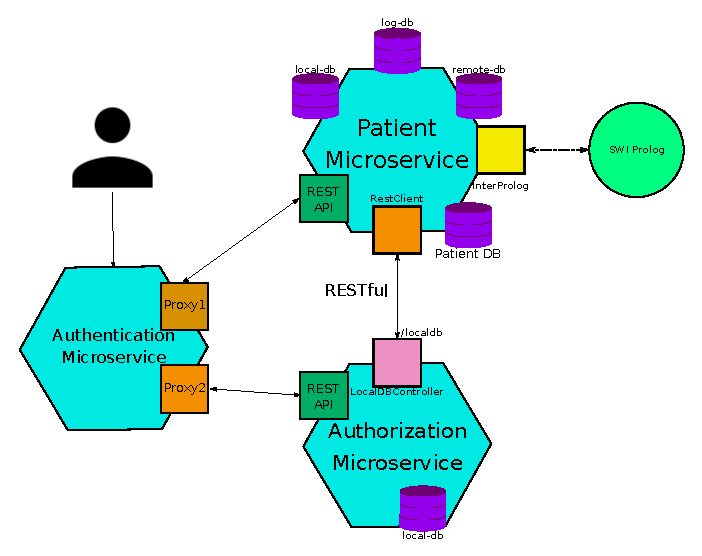
\includegraphics[width=0.45\textwidth]{./figs/mrs-mics-target.eps}}
	\caption{High-level architecture of example MRS after instrumentation by $\tool$ and $\tooll$ using the specification of Figure \ref{fig:exm-logspec}.}
	\label{fig:mrs-mics-target}
\end{figure}

$\tooll$ modifies Patient service to create an intermediary clause and communicate it with Prolog engine. Moreover, since there is a single negative trigger ($\texttt{mendTheGlass}$) a single negative trigger clause is created by the Patient service that can be used to ensure whether the preconditions are met for that negative trigger. This rule is also communicated with the Prolog engine.  Figure \ref{fig:exm-intermediary} demonstrates the intermediary and negative trigger clauses. Note that in the presentation of these rules, each method's full package/class path is redacted for brevity. 

\begin{figure}
\begin{tiny}
\begin{Verbatim}[frame=single]
/* Intermediary Clause */
lg(patient-service, getPatientMedHistory, T0,T1,[U,P]) :- 
  funccall(T0, patient-service, getPatientMedHistory, [U, P]),
  funccall(T1, authorization-service, breakTheGlass, [U]),
  <(T1, T0),
  ==(U, user).

/* Single Negative Trigger Clause */ 
negative_trigger(1,T0,T1,[U,P]) :-
  funccall(T2, authorization-service, mendTheGlass, [U]),
  <(T2, T0),
  <(T1, T2).
\end{Verbatim}
\end{tiny}
\caption{The intermediary and the negative trigger clauses for the example specification in Figure \ref{fig:exm-logspec}.}
\label{fig:exm-intermediary}
\end{figure}

Upon deciding to log an event, Patient service queries Prolog for all instances of \texttt{lg(patient-service, getPatientMedHistory, T0, T1, [U,P])} and stores the results in $\texttt{lg-list}$. Then, Patient service follows the pseudocode in Figure \ref{fig:exm-loggedcall} to infer whether logging events must be logged. Note that Figure \ref{fig:exm-loggedcall} depicts a specialization of the general process described in  \ref{fig:loggedcall}.

\begin{figure}
\begin{tiny}
\begin{Verbatim}[frame=single]
for each candidate lg(patient-service, getPatientMedHistory,T0,T1,[U,P])} 
          in lg-list:
  if negative_trigger(1,T0,T1,[U,P]) is derivable:
    LoggedCall is not derivable. Continue with the next candidate. 
  LoggedCall is derivable. Add LoggedCall(patient-service, 
                                          getPatientMedHistory,[U,P]) to log-db.
\end{Verbatim}
\end{tiny}
\caption{Example pseudocode of $\folp{LoggedCall}$ inference.}
\label{fig:exm-loggedcall}
\end{figure}





%In Section \ref{sec:intro}, we discussed an oversimplified MRS consisting of several loosely-coupled microservices. We have implemented \cite{github2} 
%a demo of this system, $\demo$, consisting of several microservices, using Java Spring Boot \cite{webb2013spring}. The front-end microservice of $\demo$ authenticates users and acts as the API gateway by relaying requests to the back-end microservices. %$\demo$ consists of the following microservices.
%
%In the following, we explain how $\demo$ is instrumented by $\tool$ for a given logging specification. In Figure \ref{fig:exm-logspec}, we have described a logging specification that enforces logging access to patient medical history at any point after breaking the glass. We can assert a similar logging specification rule in JSON \cite{github1}
%, which is more verbose than its logical equivalent. $\tool$ parses that JSON specification and constructs the Horn clause given in Figure \ref{fig:brk-horn} (ver. 1), which is then added to SWI Prolog engine fact base.
%Note that in this Horn clause presentation, we have redacted the full package names of the trigger and logging event methods and replaced them with \texttt{<package>}, for the sake of space economy.  $\tool$ instruments $\demo$ according to this logging specification rule as follows: \texttt{spring-boot-starter-aop} dependency is added to the POM of Patient and Authorization services. Authorization service is extended with  \texttt{local-db}.  Patient service is extended with \texttt{local-db}, as well as \texttt{remote-db}, and \texttt{log-db}. Authorization service is extended with the REST controller \texttt{LocalDBController} that responds to requests on path \texttt{/localdb}.  Patient service is extended with \texttt{RestClient} web client. A \textit{before} aspect is added to Authorization service with \texttt{AuthorizationController.breakTheGlass} as its pointcut. This aspect builds preconditions from the join point and appends them to \texttt{local-db}. A \textit{before} aspect is added to Patient service with pointcut \texttt{PatientController.getPatientMedHistByName}, to 1) build preconditions from the join point and append them to \texttt{local-db}, 2) send HTTP GET request on path \texttt{/localdb} to Authorization service, and store the results in \texttt{remote-db} repository,  3) add the logging specification, and contents of \texttt{local-db} and \texttt{remote-db} repositories to the SWI Prolog engine, and 4) send queries to the Prolog engine to check derivability of \texttt{loggedfunccall} predicates and accordingly update \texttt{log-db} with the engine's response.
%
%
%
%\begin{figure}
%\begin{tiny}
%\begin{Verbatim}[frame=single]
%/* Version 1 */
%loggedfunccall(T0, patient-service, 
%  "<package>.PatientController.getPatientMedHistByName", [U, P]) :-
% funccall(T0, patient-service, 
%  "<package>.PatientController.getPatientMedHistByName", [U, P]), 
% funccall(T1, authorization-service, 
%  "<package>.AuthorizationController.breakTheGlass", [U]), 
% <(T1, T0), ==(U, user).
% 
%/* Version 2 */
%loggedfunccall(T0, patient-service, 
%  "<package>.PatientController.getPatientMedHistByName", [U, P]) :-
% funccall(T0, patient-service, 
%  "<package>.PatientController.getPatientMedHistByName", [U, P]), 
% funccall(T1, authorization-service, 
%  "<package>.AuthorizationController.breakTheGlass", [U]), 
% funccall(T2, authentication-service, 
%  "<package>.AuthenticationService.authenticate", [U]), 
% <(T1, T0), <(T2, T1), ==(U, user).
% 
%/* Version 3 */
%loggedfunccall(T0, patient-service, 
%  "<package>.PatientController.getPatientMedHistByName", [U, P]) :- 
% funccall(T0, patient-service, 
%  "<package>.PatientController.getPatientMedHistByName", [U, P]), 
% funccall(T1, authorization-service, 
%  "<package>.AuthorizationController.breakTheGlass", [U]), 
% funccall(T2, patient-service, 
%  "<package>.PatientController.getAllPatients", [U]),
% funccall(T3, authorization-service, 
%  "<package>.AuthorizationController.getBTGUsers", []), 
%  <(T1, T0), <(T2, T0), <(T3, T0), ==(U, user).
%\end{Verbatim}
%\end{tiny}
%\caption{Different versions of break-the-glass policy specified as a Horn clause.}
%\label{fig:brk-horn}
%\end{figure}
%
%
%These changes describe the real-world instrumentation of the MRS, formally given in Figure \ref{fig:exm-inst}.
%Note that Authentication microservice is unaffected when instrumented by $\tool$, as it does not include any trigger or logging event methods according to the logging specification.
%
%
%
%The two other versions (Figure \ref{fig:brk-horn}) are example extensions to the policy ver. 1 . In ver. 2, authenication is considered as an additional trigger. Therefore, in addition to the aforementioned changes, $\tool$ extends Authentication microservice with  \texttt{local-db} repository, \texttt{LocalDBController}, and a \textit{before} aspect (trigger version). The \textit{before} aspect of Patient microservice is also extended with sending HTTP GET requests to Authentication microservice on path \texttt{/localdb}, and storing the results in \texttt{remote-db}. In ver. 3, two additional triggers are considered in Authorization and Patient microservices. $\tool$ applies the same changes given above, along with defining \textit{before} aspects for each extra trigger. Figures \ref{fig:mrs-mics-target} and \ref{fig:mrs-mics-target2} visually describe some of the aforementioned changes to $\demo$ by $\tool$, considering each version of the policy.%\footnote{For the sake of anonymity, we have avoided to cite the associated Github repository that includes $\tool$, $\demo$, several JSON specifications of the logging requirements and the associated instrumented versions of $\demo$. However, these implementation details can be provided by the authors if requested for reviewing purposes.}. 
%These instrumented versions are accessible in \cite{github1}, along with other examples of logging specifications, and their associated instrumented counterparts.
%
%	\begin{figure*}
%        \centering
%        \begin{subfigure}[b]{0.31\textwidth}
%            \centering
%            \fbox{
\includegraphics[width=\textwidth]{./figs/log-inst.eps}}
%            \caption[]%
%            {{\small Structure of the logging event and trigger microservices, instrumented by $\tool$.}}    
%            \label{fig:log-inst}
%        \end{subfigure}
%        \hfill
%        \begin{subfigure}[b]{0.32\textwidth}   
%            \centering 
%            \fbox{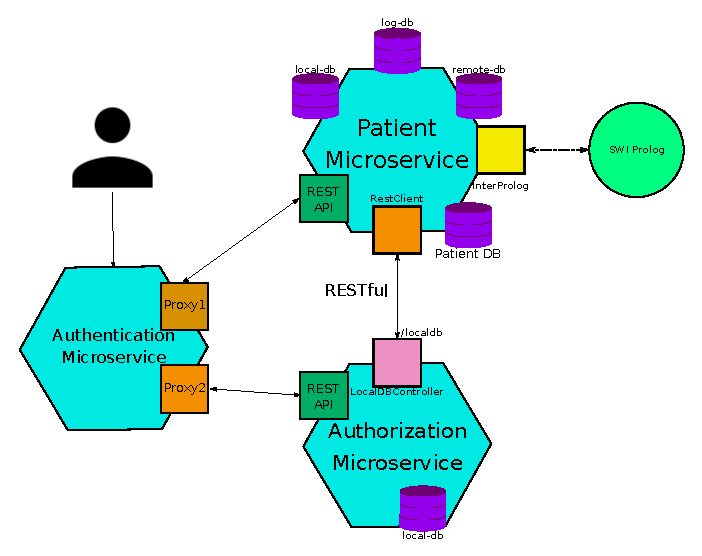
\includegraphics[width=\textwidth]{./figs/mrs-mics-target.eps}}
%             \caption[]%
%            {{\small $\demo$ instrumented by $\tool$ using versions 1 and 3 in Figure \ref{fig:brk-horn}.}}    
%            \label{fig:mrs-mics-target}
%        \end{subfigure}
%        \hfill
%        \begin{subfigure}[b]{0.32\textwidth}   
%            \centering 
%            \fbox{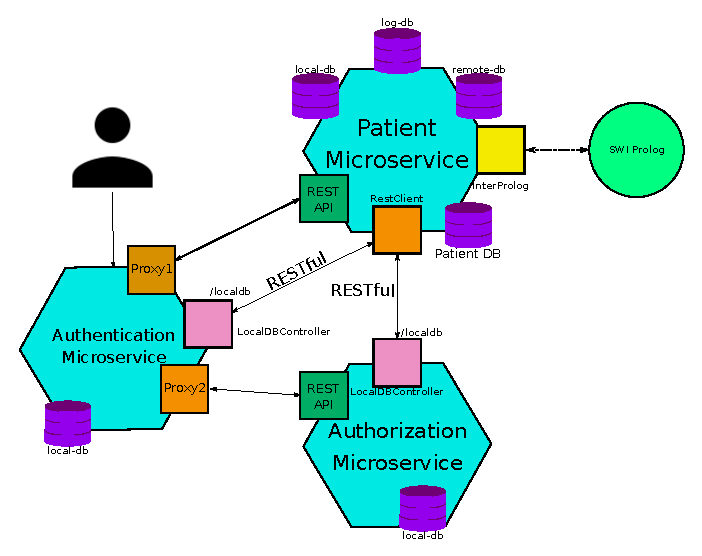
\includegraphics[width=\textwidth]{./figs/mrs-mics-target2.eps}}
%            \caption[]%
%            {{\small $\demo$ instrumented by $\tool$ using version 2 in Figure \ref{fig:brk-horn}.}}    
%            \label{fig:mrs-mics-target2}
%        \end{subfigure}
%        \vspace{5mm}
%        \caption[]
%        {\small Architecture of microservices after instrumentation.} 
%       \label{fig:mrs-structure}
%    \end{figure*}
%
%
